\documentclass{article}

% Language setting
% Replace `english' with e.g. `spanish' to change the document language
\usepackage[czech]{babel}
\usepackage[numbers]{natbib}
\bibliographystyle{plain}

\usepackage{xcolor}
\newcommand{\todo}[1]{\textcolor{red}{TODO: #1}}
% Set page size and margins
% Replace `letterpaper' with `a4paper' for UK/EU standard size
\usepackage[a4paper,top=2cm,bottom=2cm,left=3cm,right=3cm,marginparwidth=1.75cm]{geometry}

% Useful packages
\usepackage{amsmath}
\usepackage{graphicx}
\usepackage[colorlinks=true, allcolors=blue]{hyperref}

\begin{document}
  \begin{titlepage}
    \vspace*{\fill}
    \begin{center}
      {\LARGE \textbf{Projekt do předmětu KNN}}\\[0.3cm]
      {\Large \textbf{Zpracování obsahů z naskenovaných dokumentů}}\\[0.3cm]
      {\large Finální odevzdání}\\[0.5cm]
      {\large Jakub Vlk (xvlkja07)\\ Veronika Nevařilová (xnevar00)\\ Emma Krompaščíková (xkromp00)}\\
    \end{center}
    \vspace*{\fill}
  \end{titlepage}

\newpage
\section{Odkaz na repozitář}
Repozitář je k dispozici na této adrese: \href{https://github.com/vlccek/knn-project}{https://github.com/vlccek/knn-project}. V repozitáři je soubor \verb|readme.md|, který popisuje, co se kde nachází. 

\section{Definice úlohy}

Cílem tohoto zadání je vytvořit systém pro tvorbu databázových záznamů z naskenovaných stránek obsahů pro jejich jednodušší zpracování - tedy extrahovat z obrázků informace o jednotlivých kapitolách:

\begin{itemize}
    \item Název kapitoly
    \item Číslo kapitoly (pokud je k dispozici)
    \item Číslo strany
    \item Vztah kapitoly k ostatním kapitolám -- její podkapitoly (\textit{children}, viz příklad požadovaného výstupu), pokud nějaké má
\end{itemize}

Vstupem je tedy sken stránky knihy (přímo obsah, popřípadě strana, na které se nachází název nějaké kapitoly). Výstupem je soubor popisující kapitoly dané stránky ve formátu JSON. 

\begin{figure}[h]
    \centering
    \begin{minipage}{0.45\textwidth}
        \centering
        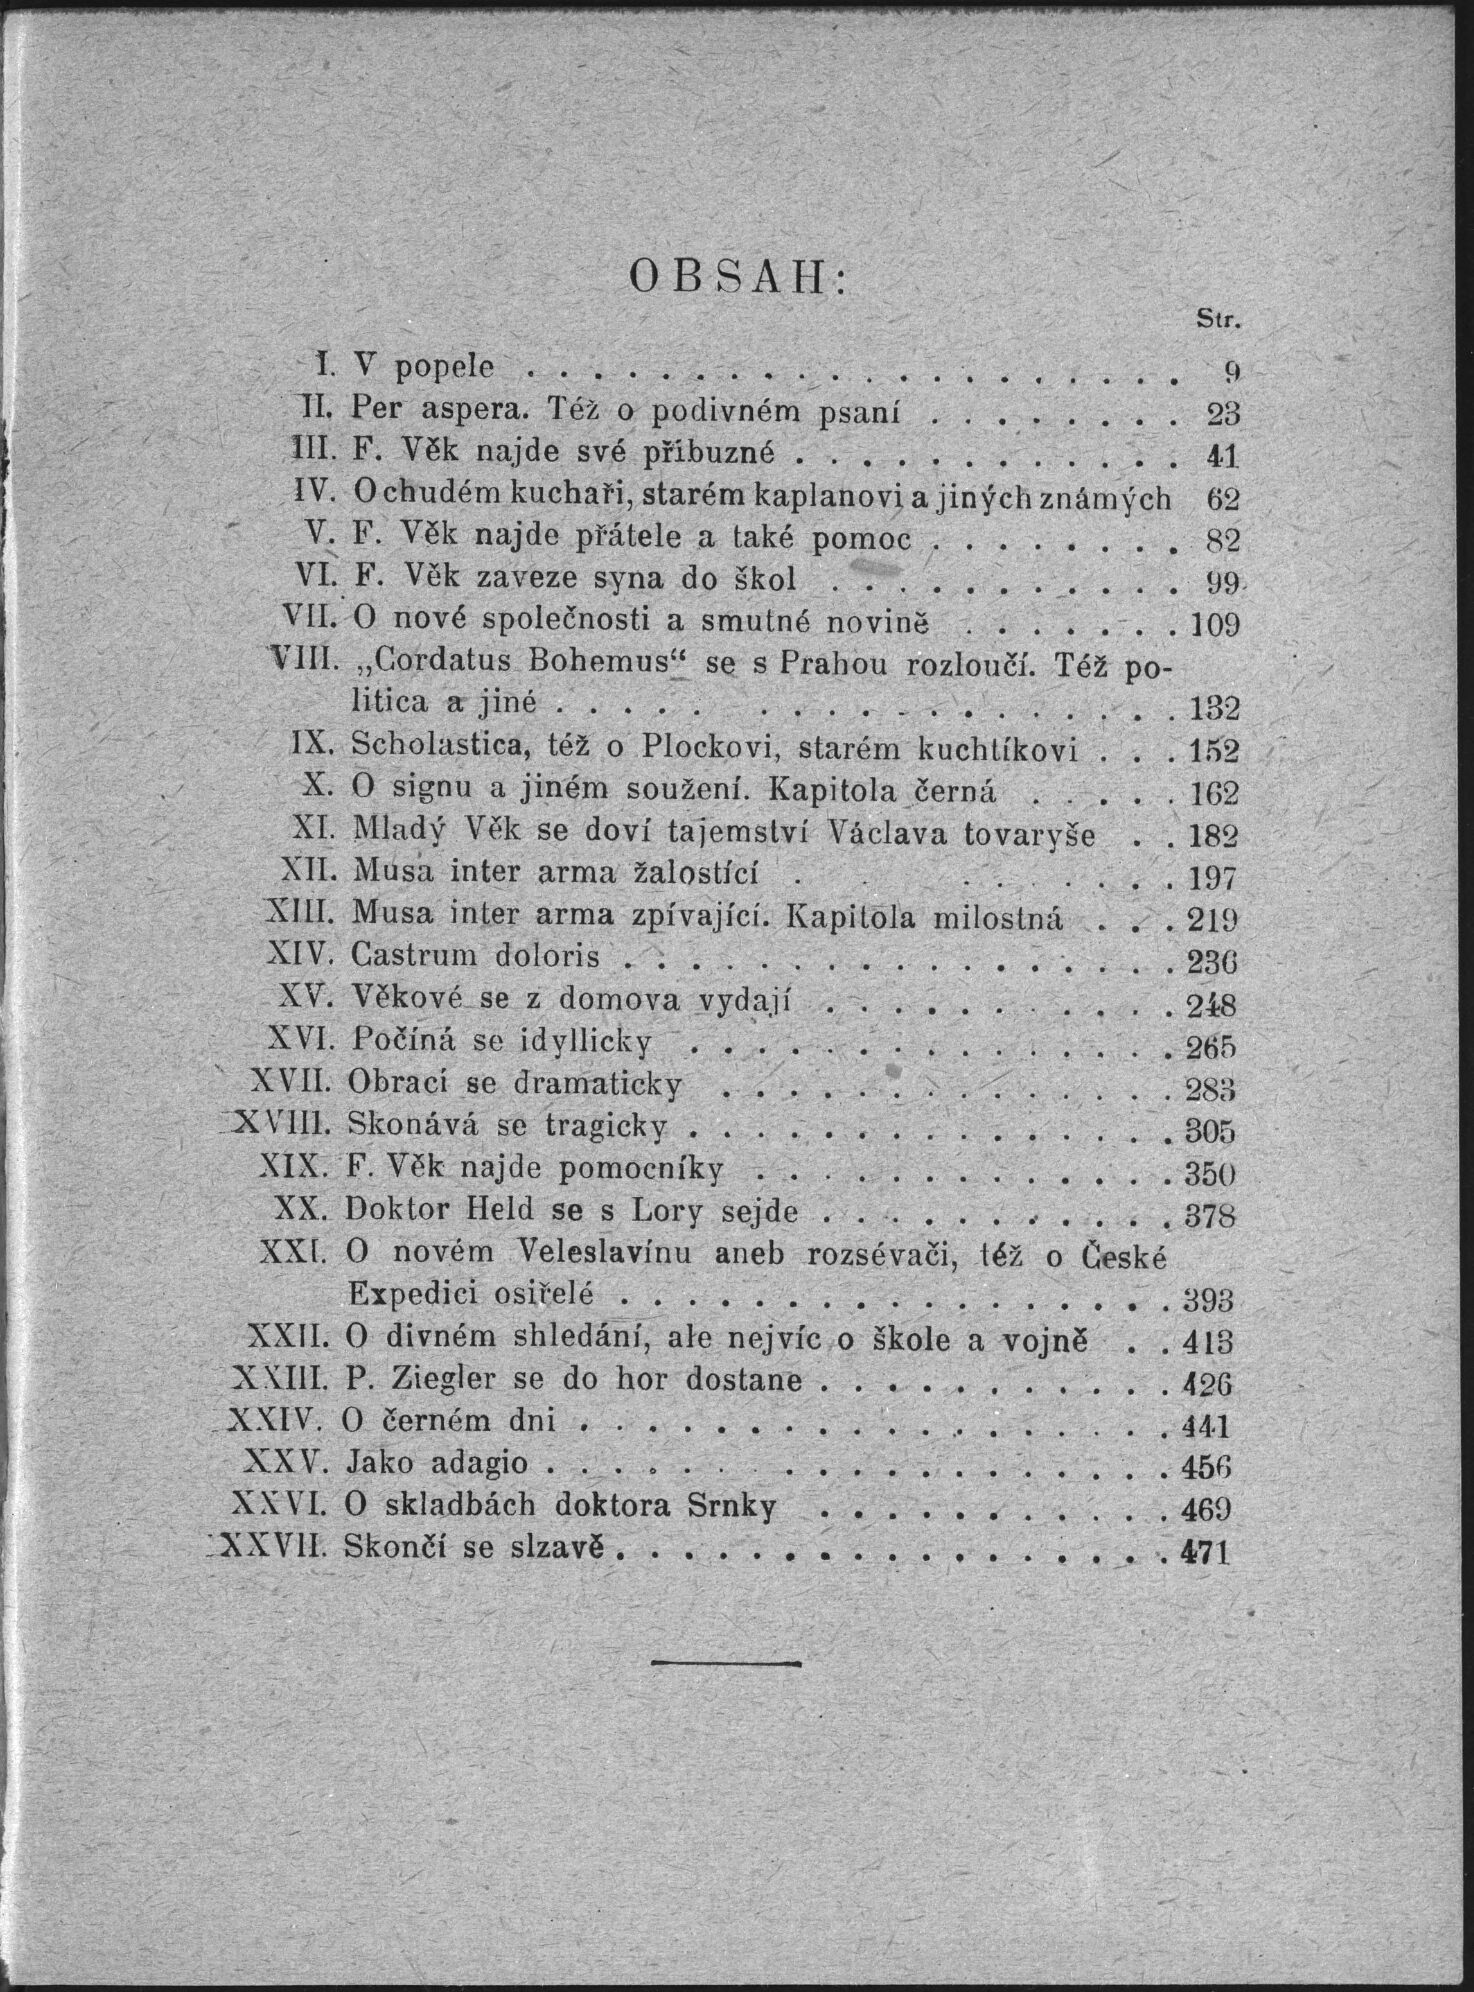
\includegraphics[width=\textwidth]{img/obsah1.jpeg}
        \caption{Příklad stránky obsahující pouze obsah.}
        \label{fig:obsah1}
    \end{minipage} \hfill
    \begin{minipage}{0.433\textwidth}
        \centering
        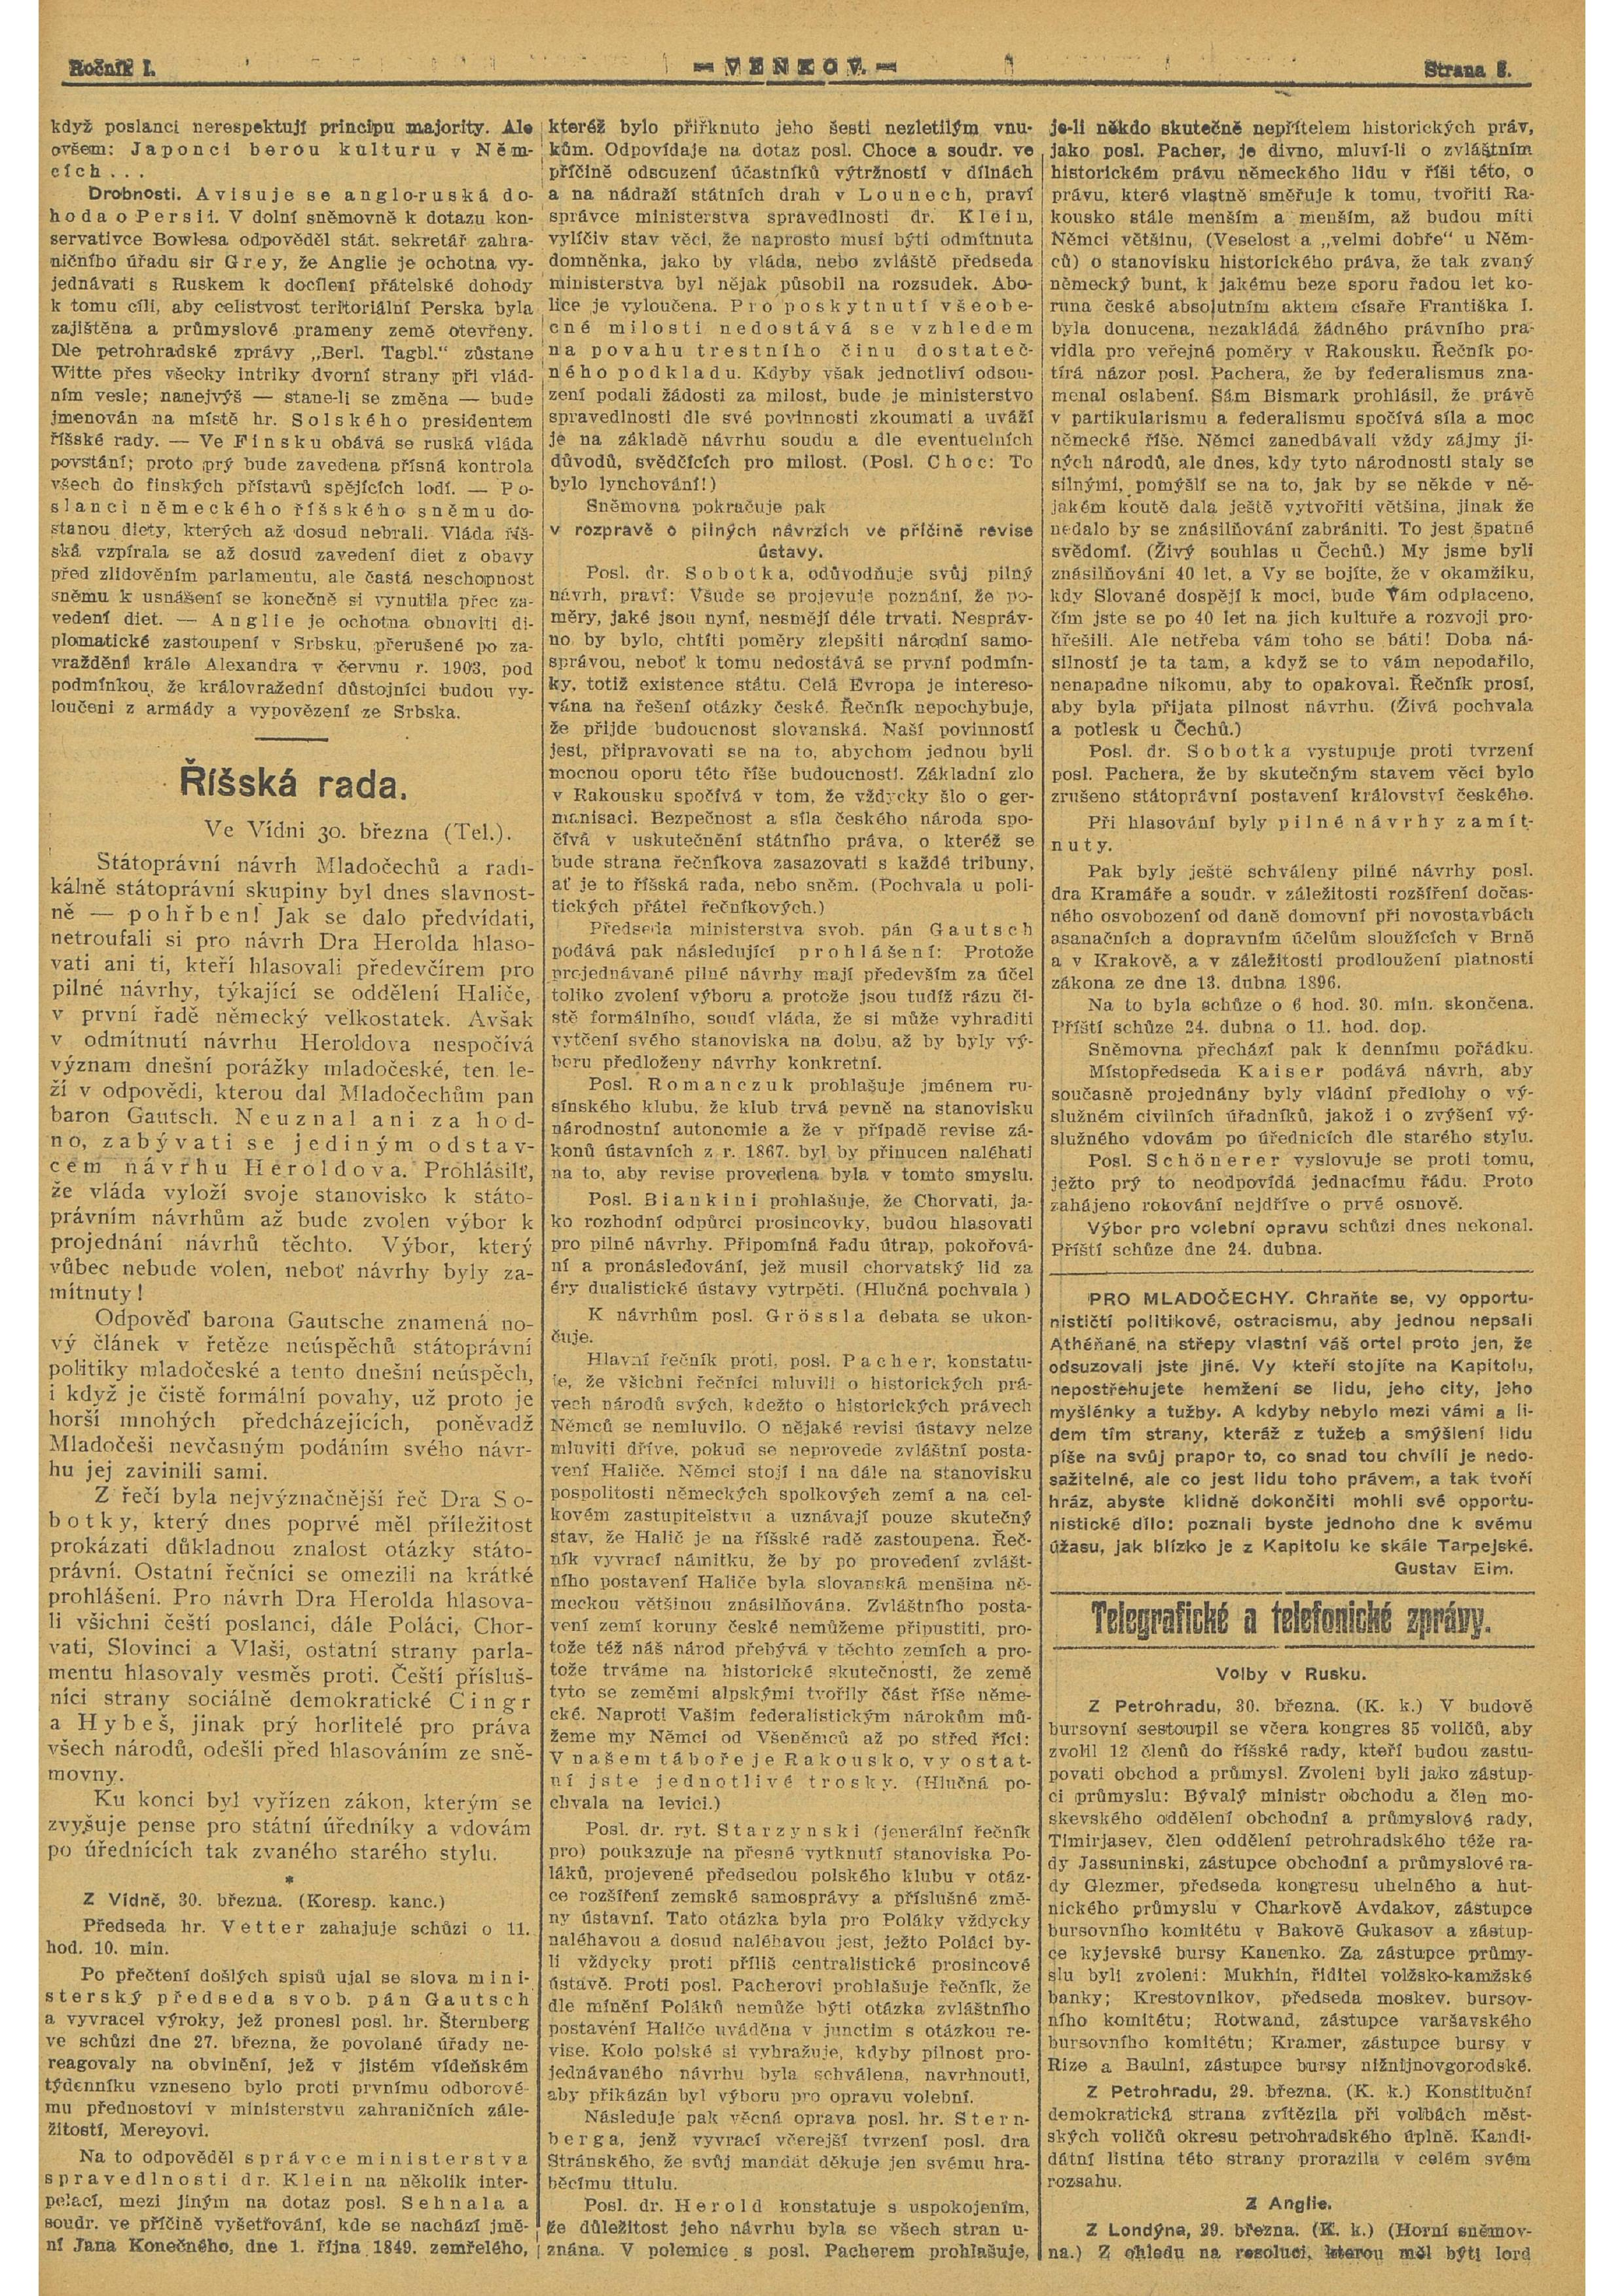
\includegraphics[width=\textwidth]{img/obsah2.jpeg}
        \caption{Příklad stránky obsahující nadpisy s textem.}
        \label{fig:obsah2}
    \end{minipage}
\end{figure}

Požadovaný výstup pro stránku z obrázku \ref{fig:obsah1} by pak vypadal následovně:

\begin{verbatim}
"result": [
  {
    "title": "V popele",
    "chapter_number": "I",
    "page_number": "9",
    "children": []
  },
  {
    "title": "Per aspera. Též o podivném psaní",
    "chapter_number": "II",
    "page_number": "23",
    "children": []
  }...
]
\end{verbatim}

\section{Existující řešení}
\label{existing_models}

Při analýze existujících řešení jsme na žádné, které by řešilo přesně naše téma, nenatrefili. Proto jsme v~této sekci sepsali řešení, která jsou našemu problému nejblíže.

\subsection{DONUT}

DONUT \cite{donut}, z angl. \textit{Document Understanding Transformer}, je end-to-end model pro porozumění dokumentů, který pro jejich zpracování nepoužívá OCR. Přímo od autorů jsou k dispozici modely DONUT přetrénované na specifické typy úloh, které zahrnují:

\begin{itemize}
\item{\textbf{Zpracování dokumentů}} -- výstupem modelu je struktura a informace extrahované z dokumentu z obrázku v digitální podobě ve formátu JSON. Tento model byl trénován na podmnožině datasetu CORD\footnote{\url{https://huggingface.co/datasets/naver-clova-ix/cord-v2}}, který obsahuje účtenky, převážně z restaurací. Dataset sestává z 800 záznamů pro train, 100 záznamů pro validation a 100 záznamů pro test množinu. Úspěšnost modelu DONUT na tomto datasetu (metrika \textit{Tree Edit Distance}) je podle oficiálního GitHub repozitáře\footnote{\url{https://github.com/clovaai/donut}} 91,3 \%.


\item{\textbf{Klasifikace dokumentů}} -- určování typu dokumentu -- např. \verb|article|, \verb|receipt| aj.

\item{\textbf{Zodpovídání otázek týkajících se dokumentů}} -- např. kolik položek na dané účtence je, nebo celková částka k zaplacení na dané faktuře.
\end{itemize}

Tento model byl také prezentován ve videu, konkrétně původní článek \textit{OCR-free Document Understanding Transformer} \cite{donut}.

\subsection{PERO OCR + LayoutLMv3}

Jedná se o řešení, které vyžaduje kombinaci dvou odlišných projektů:

\begin{itemize}
\item{\textbf{PERO OCR} -- nástroj, pomocí kterého lze automaticky přepisovat tištěný a ručně psaný text do digitální podoby spolu s dalšími informacemi \cite{pero}. Jedna z velkých výhod oproti modelu DONUT je zaměření na český jazyk.}

\item {\textbf{LayoutLMv3} -- model zpracování dokumentů pro různé účely \cite{layout}. Na jeho vstup by mělo být možné vložit výstup z PERO (text, boxy ohraničující text) a spolu s původním obrázkem dotrénovat model pro požadovaný výstup. Nevýhodou však je maximální vstupní sekvence 512 tokenů, což by pro hodně obrázků z datasetu představovalo problém.}

\end{itemize}

\section{Dataset}
Pro trénování byla obdržena od vedoucího projektu sada obrázků se skeny obsahů knih a~jiných papírových médií a anotací k nim, která není veřejné dostupná. Konkrétní datasety s požadovanými výstupy jsme si však museli vytvořit sami. Naše výsledné datasety jsou k dispozici na \href{https://drive.google.com/drive/folders/1TLxB4ENP5-d_-lFLbSLXGB39YVsoovVX?usp=sharing}{tomto} odkazu ve formátu tarballu.

\begin{figure}[htp]
    \centering
    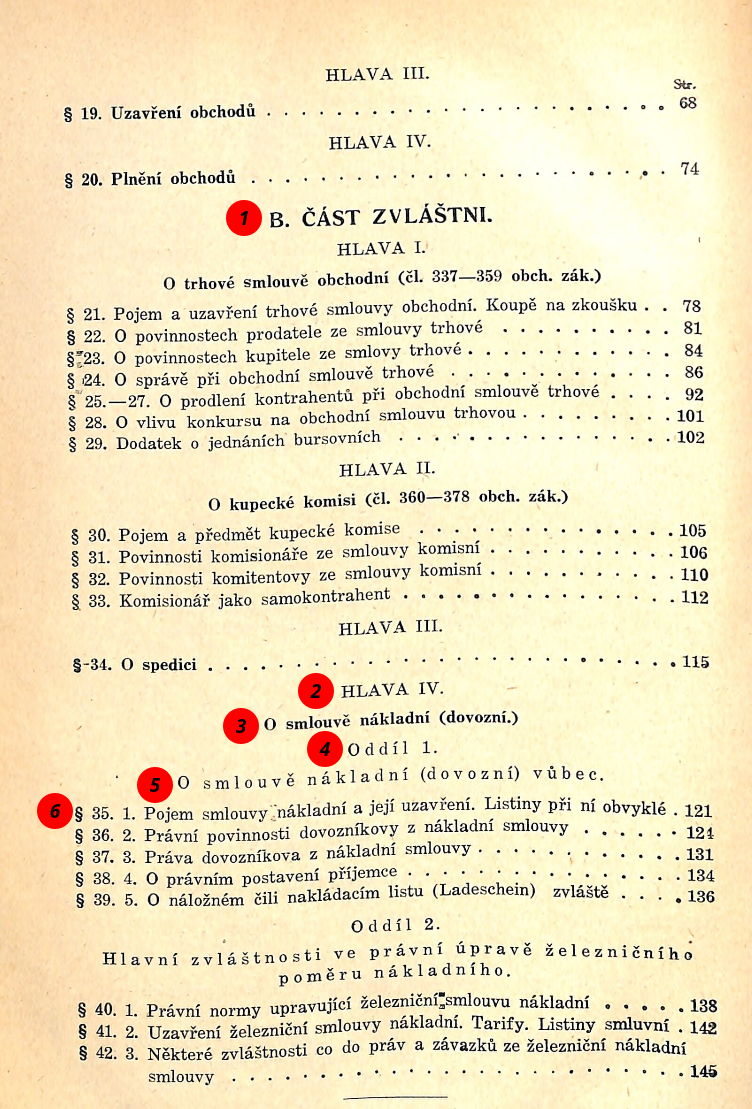
\includegraphics[width=0.4\linewidth]{img/max_rec_ilustration.png}
    \caption{Ukázka nejkomplexnějšího vzorku v rámci datasetu z hlediska množství zanoření.}
    \label{fig:enter-label}
\end{figure}

\newpage

\subsection{Poskytnuté anotace}
Anotace spočívají v označení oblastí, ve kterých se nachází jednotlivé komponenty k extrakci. Tyto anotace byly využity pro variantu PERO OCR + LayoutLMv3.  Jmenovitě dataset obsahuje:
\begin{itemize}
\item Název kapitoly (a jestli se jedná o úroveň prvního nebo jiného stupně)
\item Číslo kapitoly (pokud je k dispozici)
\item Číslo strany
\item Relace mezi kapitolou a číslem stránky 
\end{itemize}

\begin{figure}[htp]
    \centering
    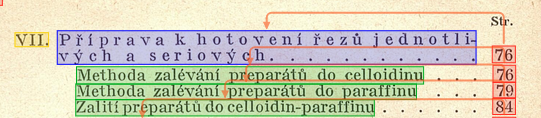
\includegraphics[width=1\linewidth]{img/anotation_show.png}
    \caption{Ukázka vizualizace anotací. Modře jsou znázorněny nadpisy hlavní úrovně, zeleně nadpisy nižší úrovně, žlutě čísla kapitol a červeně čísla stránek. Relace jsou označeny šipkami.}
    \label{fig:anotation_viz}
\end{figure}

\begin{table}[htbp]
\centering
\begin{tabular}{ll}
\hline
\textbf{Velikosti obrázků} & \\
\hline
Minimum & 500x700 px \\
Maximum & 6645x9447 px \\
Medián & 1500x2409 px \\
\hline
\end{tabular}
\caption{Informace o velikosti vstupních obrázků.}
\label{tab:dataset_info}
\end{table}


\subsection{Dataset pro DONUT}
Pro účely trénování DONUT modelu je potřeba mít připravené dvojice obrázek-očekávaný JSON. Původně jsme chtěli vytvořit JSON pomocí poskytnutých anotací. Zamýšleli jsme obrázek rozřezat podle poskytnutých anotací, na jednotlivé výřezy aplikovat OCR a tyto výsledky vložit do formátu JSONu definovaného výše. Problémem tohoto přístupu bylo, že anotace poskytují pouze relace mezi nadpisy a čísly stránek. Chyběly relace mezi úrovněmi nadpisů a také relace mezi číslem kapitoly a~nadpisem.

Tento problém by šlo vyřešit pomocí přístupu založeného na nejbližším sousedovi, ale rozhodli jsme se pro použití API velkého jazykového modelu (LLM), konkrétně Gemini\footnote{Používali jsme model \textsc{gemini-2.0-flash}, prompt je možné najít v Github repozitáři.}. Tento přístup dával tak dobré výsledky, že jsme pro později zvolený baseline model, DONUT, nepoužívali poskytnuté anotace vůbec. 



\begin{table}[htbp]
\centering
\begin{tabular}{ll}
\hline
\textbf{Kategorie} & \textbf{Detaily} \\
\hline
\textbf{Velikost datasetu} & \\
Train & 4~258 vzorků \\
Test & 541 vzorků \\
Validation & 535 vzorků \\
\textbf{Celkem} & \textbf{5~334 vzorků} \\
\hline
\textbf{Jazyky (Seřazeno dle četnosti)} & Čeština, Staročeština, Němčina, Latina, \\
 & Angličtina, Italština, Slovenština \\
\hline
\textbf{Maximální rekurze} & \\
Maximum napříč datasety & 6 \\
\hline
\textbf{Maximální počet tokenů} & 6~556 \\
\hline
\end{tabular}
\caption{Přehledová tabulka se základními informacemi o datasetu pro DONUT.}
\label{tab:dataset_info}
\end{table}

%ODKAZUJE TO V TEXTE NA TABULKU 4!!
V tabulce \ref{tab:dataset_info} jsou uvedeny základní informace o datasetu vygenerovaném pomocí LLM. Dataset obsahuje více než 5 000 vzorků rozdělených do trénovací, testovací a validační množiny, přičemž pokrývá sedm různých jazyků. Distribuci klíčových charakteristik datasetu, konkrétně hloubku rekurze a počet tokenů, lze vidět na obrázcích \ref{fig:rec_depth_histogram} a \ref{fig:token_count_histogram}. Počet tokenů je důležitý, protože model DONUT je model založený na architektuře Transformers a používá se tokenizace\footnote{Používali jsme tokenizátor pro DONUT}. 

Tento přístup i spolehlivě identifikuje stránky, na kterých nejsou obsahy. LLM vrací pro takové stránky prázdný seznam, podle promptu, který jsme zadali. Tyto stránky jsme dále pro trénování nijak nevyužili. 
\begin{figure}[htp]
    \centering
        \centering
        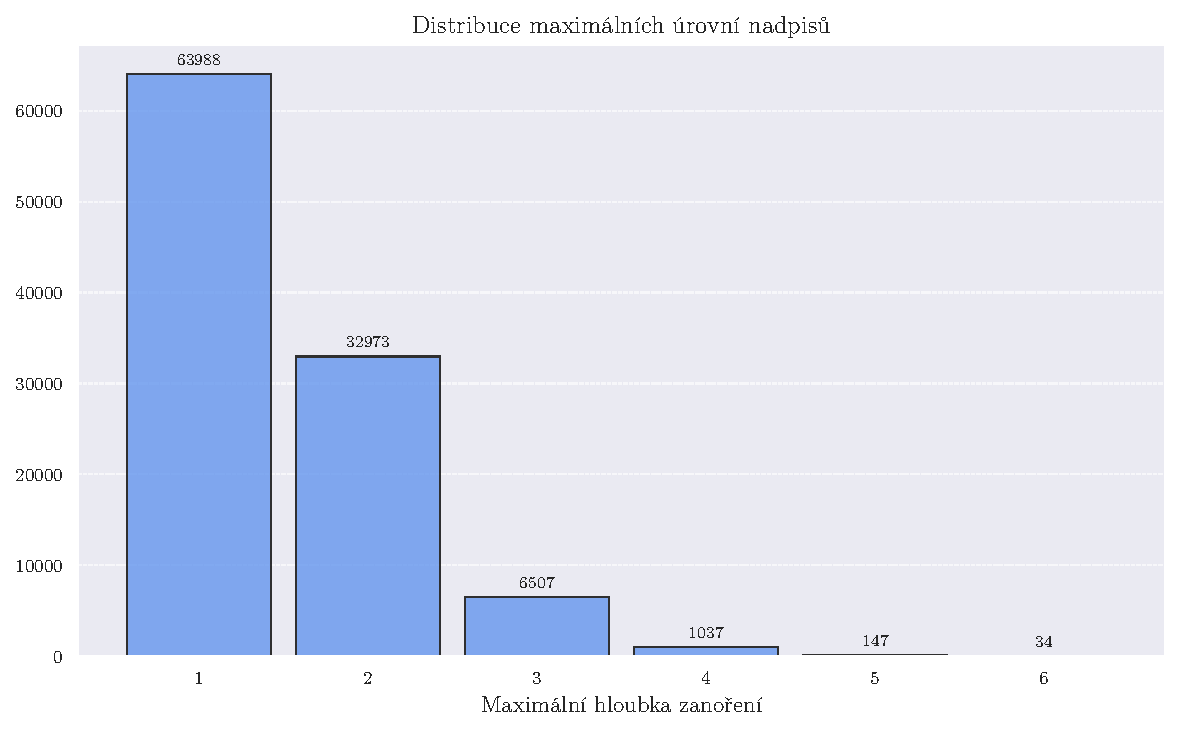
\includegraphics[width=0.74\textwidth]{img/rec_depth_histogram.pdf}
        \caption{Histogram pro maximální úroveň nadpisů. }
        \label{fig:rec_depth_histogram}
\end{figure}

\begin{figure}[htp]

        \centering
        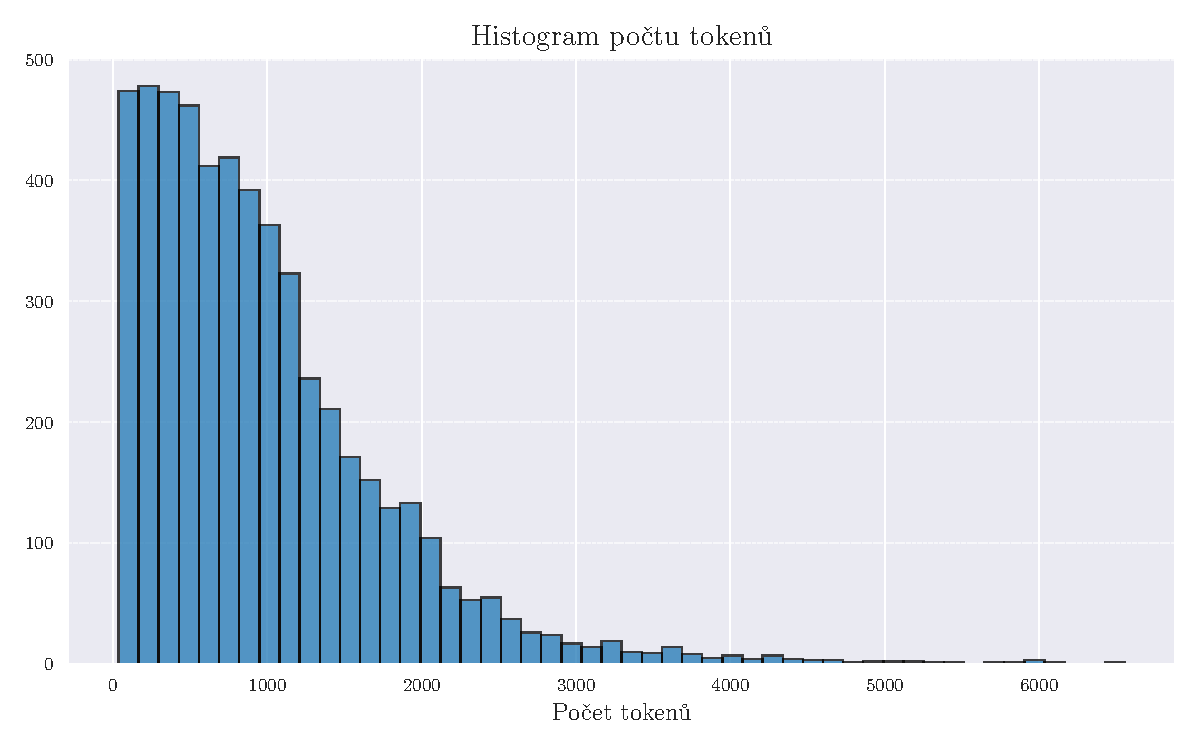
\includegraphics[width=\textwidth]{img/token_count_histogram.pdf}
        \caption{Histogram s počtem tokenů po tokenizaci.}
        \label{fig:token_count_histogram}
\end{figure}

\newpage
\subsection{Dataset pro LayoutLMv3}
Pro LayoutLMv3 jsou na vstupu potřeba jednotlivá slova, jejich bounding boxy a samotný obrázek. Očekávaným výstupem modelu je seznam klasifikací jednotlivých slov ve stejném pořadí, v jakém byla na vstupu. Pro trénování pak LayoutLMv3 vyžaduje na vstupu navíc ještě právě tyto anotace správných klasifikací. Obecně je pro trénování potřeba dataset ve formátu:

\begin{figure}[htp]
% 05f9c8ec-755a-4257-a532-c52ee755ddbc.6.6e5ca56d-7517-4794-bfda-9760a5b0c594.jpg
    \centering
    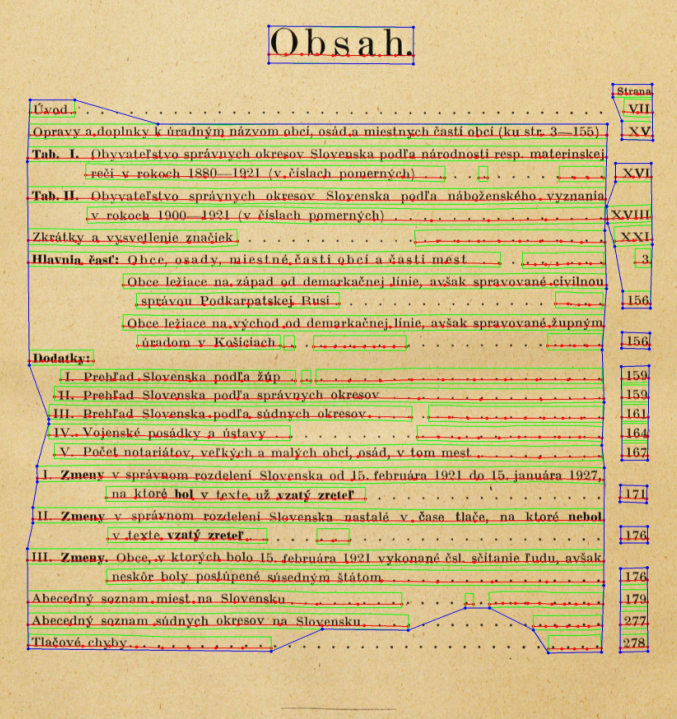
\includegraphics[width=0.75\linewidth]{img/pero-ocr-example.png}
    \caption{Vizualizace ALTO formátu. Lze vidět ohraničení pro části textu, řádky a slova.}
    \label{fig:pero-exampleoutput}
\end{figure}

\begin{verbatim}
[
  {
    "tokens": ["V", "popele",...],
    "bboxes": [[392, 367, 549, 392],[142, 418, 165, 440],...],
    "ner_tags": [1,0,...],
    "image": "path/to/image.jpg"
  }...
]
\end{verbatim}

V \verb|ner_tags| jsme použili mapování jednotlivých tříd stejných jako v dodaných ručních anotacích na celá čísla:

\begin{verbatim}
"trash": 0
"kapitola": 1
"cislo strany": 2
"jiny nadpis": 3
"jine cislo": 4
"podnadpis": 5
"nadpis v textu": 6
\end{verbatim}

Kromě tříd vyskytujících se v ručních anotacích jsme pak přidali ještě speciální třídu \verb|trash| s hodnotou 0, která vyjadřuje slova, která jsou pro vytváření obsahu nedůležitá (dodatky na konci strany či jiný text nepředstavující část obsahu).

Na doporučení vedoucího jsme použili nástroj PERO\footnote{\url{https://github.com/DCGM/pero-ocr}}, jehož výstupem jsou mimo jiné také soubory ve formátu ALTO (Analyzed Layout and Text Object). Vizualizaci takového souboru lze vidět na obrázku \ref{fig:pero-exampleoutput}. Jedná se o standardní XML formát pro popis rozložení a obsahu digitalizovaných dokumentů, včetně umístění textových bloků, řádků a slov, a rozpoznaného textu. Z tohoto souboru lze získat požadované informace, konkrétně jednotlivá slova a jejich bounding boxy (BB).
\newpage
Celý proces vytváření datasetu tedy probíhal takto:

\begin{enumerate}
    \item{Zpracování obrázků pomocí PERO}
    \item{Převod černobílých obrázků na RGB formát (LayoutLMv3 vyžaduje RGB obrázky)}
    \item{Zpracování ALTO výstupů a převod souřadnic na souřadnice kompatibilní s těmi z ručních anotací}
    \item{Porovnání bounding boxů jednotlivých slov s ručními anotacemi - daný bounding box byl klasifikován stejnou třídou, jakou má bounding box z ručních anotací, se kterou se nejvíce překrýval. Pokud se nepřekrýval s žádným boxem z anotací, znamená to, že dané slovo není částí obsahu a je tedy klasifikováno jako třída \verb|trash|.}
    \item{Normalizace souřadnic bounding boxu - LayoutLMv3 akceptuje souřadnice v rozmezí hodnot 0-1000}.
\end{enumerate}

Vzhledem k tomu, že u tohoto přístupu jsme na rozdíl u Donutu byli omezeni počtem obrázků, který byl anotován, po vyřazení některých nevalidních vzorků (obrázky s obsahem zanořeným více než 2 úrovně, anotace s neodpovídajícími rozměry obrázku vůči rozměrům uvedeným ve výstupech z PERO) má výsledný dataset pouze okolo 1000 obrázků se zvoleným poměrem množin \verb|80:10:10|:
\begin{table}[htbp]
\centering
\begin{tabular}{lc}
\hline
\textbf{Množina datasetu} & \textbf{Počet vzorků} \\
\hline
Train & 784 \\
Test & 98 \\
Validation & 98 \\
\hline
\textbf{Celkem} & 980 \\

\hline
\end{tabular}
\caption{Velikost jednotlivých množin datasetu.}
\label{tab:dataset_info}
\end{table}

\section{Použité metriky}
Převzali jsme metriky, které používali autoři původního modelu DONUT pro evaluaci modelu pro zpracování účtenek, což je typ úkolu nejvíce podobný našemu. Jedná se o metriky \textit{Tree Edit Distance} a~\textit{F1}.

\subsection{Normalizovaná Tree Edit Distance přesnost}
Pro vyhodnocení strukturální podobnosti mezi predikcí modelu a očekávaným výstupem jsme využili normalizovaný Tree Edit Distance (TED). TED sama o sobě počítá minimální počet operací (vložení, smazání a substituce uzlů), které jsou potřeba k transformaci jednoho stromu na druhý. V našem případě jsou při testování DONUT modelu převedeny vygenerované JSON struktury na stromy, kde každý uzel reprezentuje jednu položku obsahu. Nižší hodnota TED značí větší podobnost mezi predikcí a referenčním výstupem, což naznačuje lepší schopnost modelu zachytit hierarchickou strukturu obsahu dokumentu. Normalizace podle velikosti referenčního stromu a odčítání této hodnoty od 1~pak představuje přesnost modelu pohybující se v hodnotách od 0 do 1. Tuto konkrétní metriku proto maximalizujeme.

\[
\text{NormedTEDAcc} = \max\left(0,\ 1 - \frac{\text{TED(prediction, answer)}}{\text{TED}(\emptyset,\ \text{answer})}\right)
\]

\subsection{F1 skóre}
\label{f1}
Jako doplňkovou metriku jsme použili F1 skóre, které poskytuje vyvážený pohled na přesnost a úplnost extrakce. F1 skóre je harmonický průměr mezi precision (přesnost) a recall (úplnost), kde precision představuje podíl správně identifikovaných položek v predikci a recall představuje podíl referenčních položek, které byly úspěšně predikovány. Tato metrika je důležitá pro vyhodnocení schopnosti modelu korektně extrahovat všechny relevantní komponenty obsahu (nadpisy, čísla stránek, čísla kapitol) bez falešných detekcí. Vyšší hodnota F1 skóre indikuje kvalitu extrakce obsahů a tuto metriku proto rovněž maximalizujeme. Hodnoty taktéž náleží do intervalu od~0~do~1.

\[
\text{F1} = \frac{2 \cdot \text{precision} \cdot \text{recall}}{\text{precision} + \text{recall}}
\]

Je také potřeba zmínit, že evaluace modelu DONUT v kódu probíhá tak, že se vyhodnocuje hodnota F1 skóre na výsledcích predikce jednotlivých obrázků. Nejmenší jednotka tohoto vyhodnocení je tedy celá predikce jednoho obrázku. Pokud je predikce naprosto stejná s požadovaným výsledkem, je to klasifikováno jako \textit{true positive}. Pokud se v predikci liší byť jen jeden znak, je predikce označena za \textit{false positive} nebo \textit{false negative}, v závislosti na situaci.

\section{Baseline řešení}

Jako baseline řešení jsme z možností zmíněných v sekci \ref{existing_models} zvolili model DONUT z důvodů:

\begin{itemize}
\item{\textbf{End-to-end řešení} -- není potřeba spojovat více modelů za sebe}
\item{\textbf{Trénovaný na velmi podobný typ úkolu} -- přetrénovat CORD verzi na náš požadovaný výstup by mělo být možné, a díky tomu, že model byl přetrénován na podobném úkolu, nebude pravděpodobně potřeba mít obrovský dataset -- model již bude umět zpracovávat obrázek, co se zanoření a určování prvků v obrázku týče}

\item{\textbf{Úspěšnost v přetrénovávání modelu na podobných úkolech} -- při hledání informací o~modelu jsme natrefili na spoustu internetových diskuzí, kde použití CORD DONUT modelu pro specifická řešení vývojáři chválili}

\item{\textbf{Existující trénovací a testovací skripty} -- autoři ve svém GitHub repozitáři poskytují skripty pro práci s modelem}
\end{itemize}

DONUT má řadu nevýhod, které mohou trénování ztížit nebo přímo znemožnit, mezi které patří zejména to, že \textbf{nebyl trénován na českém jazyce}. DONUT byl trénován pouze na angličtině, japonštině, čínštině a korejštině. Zkusili jsme proto originálnímu modelu verze CORD předložit některé obrázky z našeho datasetu a ten nepřekvapivě přepisoval všechny znaky obsahující interpunkci bez ní. Každopádně v tokenizeru modelu jsme našli pár českých znaků, a proto jsme se i přesto trénování rozhodli vyzkoušet.

\subsection{Dataset pro DONUT}

Architekturu datasetu jsme doladili podle požadavků GitHub repozitáře DONUT modelu. Dataset se skládá ze tří adresářů, \textbf{train}, \textbf{validation} a \textbf{test}, přičemž každý adresář obsahuje soubor \verb|metadata.jsonl|, ve kterém se nachází dvojice \verb|file_name| a \verb|ground_truth| pro každý obrázek z~daného datasetu. Ve stejném adresáři se pak nachází také všechny obrázky zmíněné v metadatech. Jako \verb|ground_truth| jsme použili přímo požadované JSON výstupy modelu ve formě textového řetězce.

\subsection{Trénování}

Pro trénování jsme si vytvořili účty na Metacentru\footnote{\url{https://metavo.metacentrum.cz/}}. DONUT totiž potřebuje pro trénování velký objem GPU paměti, a proto lokální trénování nebylo možné.

I přesto, že samotné trénování mělo být poměrně jednoduché, jsme natrefili na spoustu problémů, které nakonec vyústily ve velké změny celého kódu DONUT repozitáře. Trénování jsme úspěšně zprovoznili, ale i přesto, že model v průběhu trénování vykazoval známky učení a zlepšování se, měl po natrénování vždy mnohem horší úspěšnost než měl jeho koncový stav trénování. Tento problém je (dle množství vytvořených issues s tímto tématem na DONUT GitHubu) poměrně častý a~neexistuje univerzální postup, kterým by se vyřešil. Museli jsme proto upravovat kód, instalovat různé verze balíčků a zkoušet různá nastavení trénování. Nakonec se však kód podařilo dostat do bodu, kdy trénování začalo mít mnohem lepší výsledky.

Před našimi úpravami trvalo i 15 epoch modelu, aby začal rozpoznávat strukturu požadovaného výstupu v obrázcích. V aktuální verzi již po jedné epoše vykazuje orientaci v tom, jakou úlohu má plnit a správně dokáže například spojit název kapitoly a číslo její strany.

Další věcí, která nás mile překvapila, bylo naučení správného rozpoznávání českých znaků a textů, s čímž model po pár epochách neměl žádný větší problém.

Zezačátku jsme zkoušeli model trénovat na 8 epochách, a po nich již model bez problému dokáže některé obrázky zpracovat se 100\% úspěšností.

\subsection{Vyhodnocení baseline}

Vyhodnocovat původní DONUT model CORD na našich datech nemělo smysl. Daný model je totiž naučen na účtenkách, a proto i pokud našel v našich datech nějaký vzor, výstupní JSON absolutně neodpovídal našemu požadovanému výstupu a obě metriky by očividně měly hodnotu 1. Proto jsme model vyhodnotili po přetrénování, abychom měli relevantní výsledky.

Vyhodnocení jsme provedli standardní inferencí na modelu. Použili jsme testovací dataset. Výsledné hodnoty TED a F1 po natrénování byly:


\begin{table}[htp]
\centering
\begin{tabular}{c||cc}
\hline
\textbf{Počet epoch} & \textbf{Norm. tree edit distance přesnost} & \textbf{F1 skóre} \\
\hline
8 & 0.70 & 0.39 \\
\hline
\end{tabular}

\caption{Tabulka s výsledky inference na modelu vztažených k počtu epoch.}
\label{tab:dataset_info}
\end{table}

Tyto prozatimní výsledky vnímáme pozitivně,  vzhledem k tomu, že jsme čelili problémům s baseline řešením a zatím jsme tedy nemli možnost vyladit různé konfigurace modelu a vyzkoušet více epoch. Pouhých 8 epoch stačilo modelu, který nebyl předtím trénován na českém jazyce, aby začal přepisovat naše skeny obrázků s přesností norm. TED 70 \% a F1 39 \%. \footnote{Model je nahrán na Google Drive: \url{https://drive.google.com/drive/folders/1wHiaRq4rd3egE_rcKunOHjj6pBsMckQd?usp=sharing}.}

\subsection{Vývoj loss}
Z průběhu loss funkce na obrázku \ref{fig:loss_func} jde vidět, že by určitě šlo model ještě trénovat a její hodnoty stále lehce klesají. Loss funkce vykazuje zdravé učení.

\begin{figure}[htp]
    \centering
    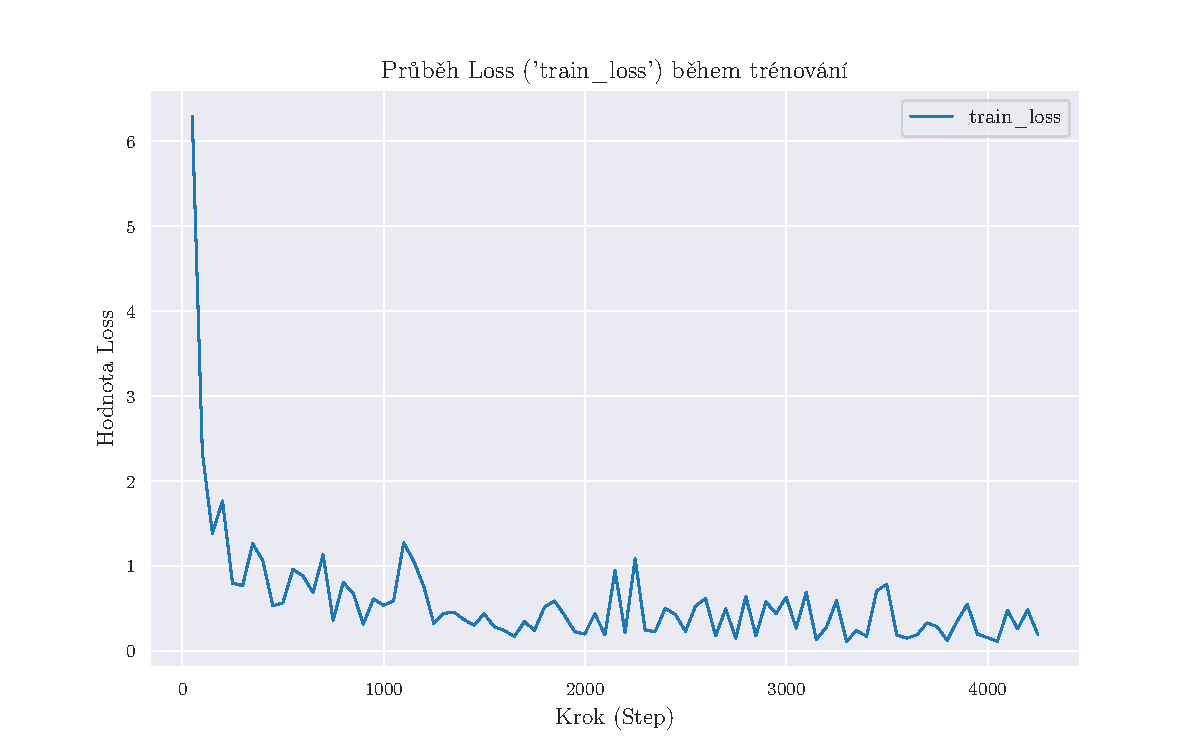
\includegraphics[width=1\linewidth]{img/train_loss.pdf}
    \caption{Vývoj loss funkce v průběhu trénování.}
    \label{fig:loss_func}
\end{figure}

\subsection{Úpravy baseline po checkpointu}
Po odevzdání checkpointu jsme provedli ještě několik experimentů s cílem vylepšit přesnost modelu. Vyfiltrovali jsme dataset tak, aby obsahoval jen nadpisy druhé úrovně. Experimentovali jsme také s počtem epoch, který jsme tentokrát nastavili na $25$. Výsledky se nám podařilo mírně vylepšit, jak je vidět v tabulce \ref{tab:dataset_info_2}. Provedli jsme i ruční kontrolu výstupu jazykového modelu a kontrola ukázala, že většina kontrolovaných vzorků byla zcela bezchybná. U malé části vzorků, které vykazovaly určité nedostatky, jsme identifikovali několik hlavních kategorií chyb.

Přibližně třetinu těchto problémových vzorků tvořily chyby v interpunkci. Jednalo se především o chybějící tečky za římskými čísly, ale zaznamenali jsme i nesprávné použití či absenci pomlček a spojovníků, nebo nadbytečná interpunkční znaménka.

Podobně časté, rovněž s podílem přibližně jedné třetiny problémových vzorků, byly strukturální nesrovnalosti. Zde jsme narazili na extrakci nadbytečných dat, typicky v podobě nadbytečných čísel stran, která nepatřila k danému záznamu, nebo i celých řádků obsahu, které do extrahovaných informací nepatřily. Naopak, v některých případech chyběly relevantní části textu kapitol. Specifickým problémem byla také občasná mylná extrakce slova "OBSAH" jako názvu kapitoly. Jako méně častá, avšak docela závažná chyba, byly posunuté čísla stránky obsahu o jeden řádek nahoru, kdy došlo k chybnému strukturálnímu přiřazení celého obsahu stránky.

Menší podíl tvořily problémy související s optickým rozpoznáváním znaků a zpracováním textů. Zde jsme zaznamenali nesprávně rozpoznané znaky, zejména s diakritikou (např. SIRÉNA rozpoznáno jako SIRENA), záměnu písmen (např. D jako O), či potíže při zpracování cizojazyčných kaligrafických německých textů, kde bylo náročné zjistit, zda je okrasné písmo rozpoznáno správně.. Problém představoval i ručně psaný text, který nebyl spolehlivě rozpoznán.

Nakonec, s podílem okolo 5--10\,\% problémových vzorků, se objevovaly chyby při spojování slov, která byla v obsahu rozdělena na konci řádku.

I přesto je však, vzhledem ke způsobu, jakým je počítána hodnota F1 v evaluačním skriptu modelu DONUT (popsána v sekci \ref{f1}), tato hodnota poměrně vysoká a znamená poměrně přesné zpracování obsahů stran.

\begin{table}[ht]
\centering
\begin{tabular}{c||cc}
\hline
\textbf{Počet epoch} & \textbf{Norm. tree edit distance přesnost} & \textbf{F1 skóre} \\
\hline
25 & 0.75 & 0.42 \\
\hline
\end{tabular}
\caption{Tabulka s výsledky inference na modelu vztažených k počtu epoch v druhé části semestru.}
\label{tab:dataset_info_2}
\end{table}


\section{PERO-LayoutLMv3}

Projekt byl pojat jako porovnání dvou odlišných přístupů k řešení daného problému. První z nich, založený na modernějších principech Transformerů, který byl prezentován v rámci checkpointu, vyžaduje náročnější anotace. Jejich ruční vytvoření by bylo velmi drahé a náchylné k chybám, a proto jsme se rozhodli je vygenerovat pomocí jazykového modelu. Tímto postupem se de facto destilují znalosti LLM, bohužel však s tím se přenášejí i jeho chyby.

Druhý přístup sice rovněž vyžaduje anotace, ale jejich tvorba je jednodušší než vytvoření kompletního JSONu s úrovněmi a kompletním přepisem potřebným pro první přístup.

Celkově lze říci, že přístup založený na PERO a LayoutLMv3 klade menší nároky na přímou anotaci člověkem (případně se zbavuje závislosti na LLM), ale za to je potřeba vynaložit více úsilí na komplexnější práci se vstupy a výstupy modelu.

\subsection{Trénování LayoutLMv3}

Základ trénovacího skriptu byl převzat z GitHubu Hugging Face\footnote{\url{https://github.com/huggingface/transformers-research-projects/blob/main/layoutlmv3/run_funsd_cord.py}}, který byl dále upraven pro potřeby tohoto projektu. Vzhledem k velké vytíženosti Metacentra a faktu, že LayoutLMv3 ne\-vy\-ža\-du\-je příliš velký výpočetní výkon, trénování tentokrát oproti Donutu probíhalo na Google Colab\footnote{{\url{https://colab.research.google.com/}}} formou Jupyter notebooku. Trénování probíhalo několikrát s různým nastavením hyperparametrů. Nejvyšší přesnosti bylo však dosáhnuto při trénování 10 epoch a learning rate $5 \cdot 10^{-5}$. Při vyšším počtu epoch či větší learning rate již docházelo u modelu k přetrénování. Pro evaluaci při i po trénování bylo využito metriky F1. Trénováním bylo dosáhnuto maximální hodnoty F1 na testovací sadě
75,7 \%. Vývoj hodnot loss funkce a F1 skóre je zobrazen v obrázku \ref{layout_training}, kde jsou v grafu vyneseny pro srovnání dva vybrané běhy trénování s různým nastavením learning rate, $5 \cdot 10^{-5}$ (oranžově, výsledný zvolený model) a $1 \cdot 10^{-4}$ (červeně).

\begin{figure}[h]
    \centering
    \begin{minipage}{0.5\textwidth}
        \centering
        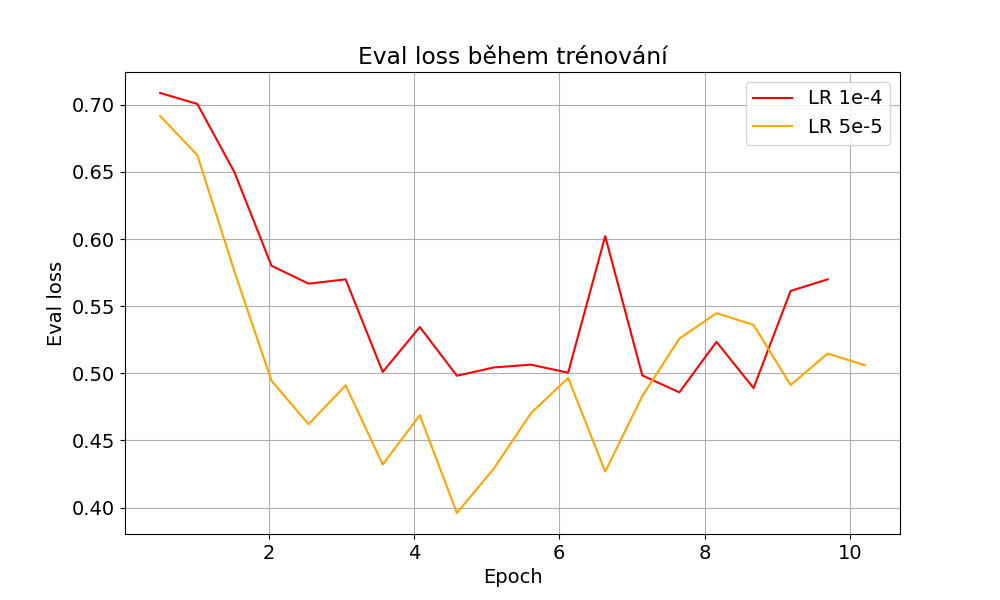
\includegraphics[width=\textwidth]{img/loss_plot.png}
    \end{minipage}\hfill
    \begin{minipage}{0.5\textwidth}
        \centering
        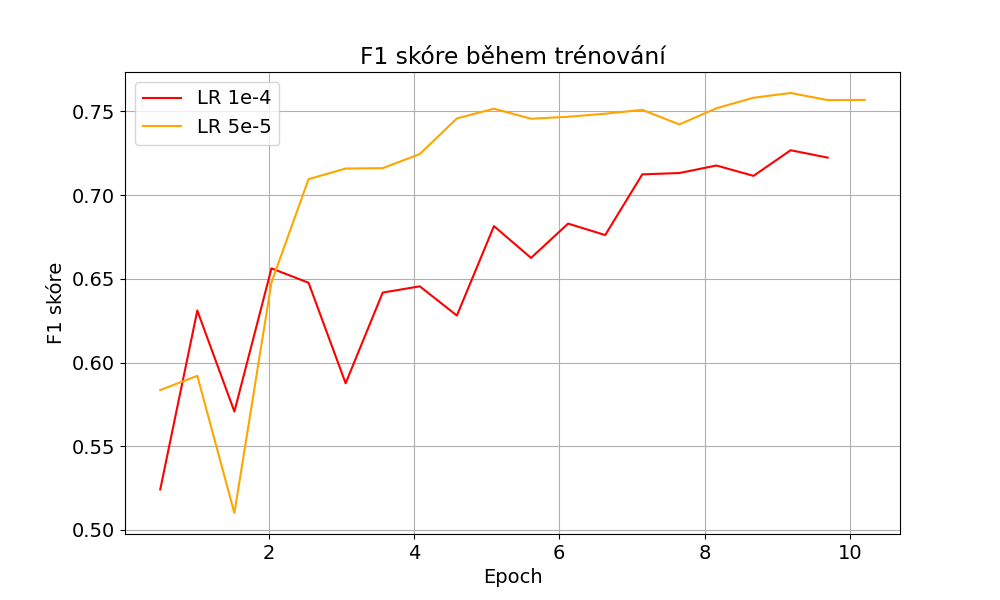
\includegraphics[width=\textwidth]{img/f1_plot.png}
    \end{minipage}
    \caption{Vývoj hodnot loss funkce a F1 skóre na evaluační sadě behem trénování s různým nastavením hodnot learning rate.}
    \label{layout_training}
\end{figure}

Po úspěšném natrénování LayoutLMv3 bylo již možné přejít ke spojení všech nástrojů ve formě výsledného kódu pro zpracování jednotlivých obrázků.


\subsection{Pipeline pro inferenci}
Výsledný kód pro zpracování by měl být co nejvíce uživatelsky přívětivý a jednoduchý. Vstupem by tedy ideálně měl být pouze daný obrázek, který uživatel chce převést na obsah, a výstupem by měl být již samotný obsah ve formátu JSON.

\subsubsection{Spuštění}
Soubor \verb|run.sh| pro spuštění tohoto výsledného kódu je umístěn v \verb|pero_layout/pipeline|. Obrázek, jehož obsah chce uživatel převést na JSON, musí být umístěn ve složce \verb|images|. Dále se ve složce musí nacházet složky obsahující PERO a LayoutLMv3. Skript se spouští pouhým příkazem \verb|./run.sh| (podrobný návod pro spuštění je přiložen v \verb|readme.md|). Celé zpracování daného obrázku probíhá ve třech základních krocích popsaných níže.

\subsubsection{Získání OCR výstupů pomocí PERO}

V první části skript zavolá PERO pro zpracování daného obrázku v adresáři \verb|images|. Všechny výstupy z PERO jsou uloženy v adresáři \verb|output|. Pro další zpracování však jsou použity pouze výstupy ALTO.

\subsubsection{Převod OCR výstupů do formátu kompatibilního s LayoutLMv3}

Dále se spustí soubor \verb|ocr-to-json.py| nacházející se v adresáři \verb|processing|, kterému jsou předány dva argumenty -- adresář s výstupy PERO a adresář obsahující původní obrázek. Tento skript spustí převod výstupů z PERO do formátu, který přijímá LayoutLMv3, pomocí třídy \verb|PeroProcessor|. Ta funguje podobně jako skript pro přípravu datasetů -- převede výstup OCR na pole jednotlivých slov, jim odpovídající normalizované bounding boxy, a předá také cestu k danému původnímu obrázku. Všechna potřebná data jsou tedy vrácena jako slovník s klíči \verb|bboxes|, \verb|tokens|, \verb|image_path|.

\subsubsection{Inference pomocí LayoutLMv3}
Data popisující daný obrázek jsou předána třídě \verb|LayoutProcessor|, která provede načtení na\-tré\-no\-va\-né\-ho modelu a inferenci obrázku. Následně je ještě provedeno zpracování, kdy se např. odstraní okrajové výplně výstupů či se spojí podslova jednotlivých slov. Pro kontrolu správnosti je ještě přidán kód, který jednotlivá klasifikovaná slova v obrázku označí a připíše k nim jejich klasifikovanou třídu. Tento bod slouží především k ověření, že celé zpracování probíhá korektně. Příklad takto zpracovaného obrázku je zobrazen v obrázku \ref{fig:layout-output}. Výstupem tohoto kroku je tedy pole klasifikovaných slov ve stejném pořadí, jako byly modelu předány, a níže zobrazený obrázek.

\begin{figure}[ht]
    \centering
    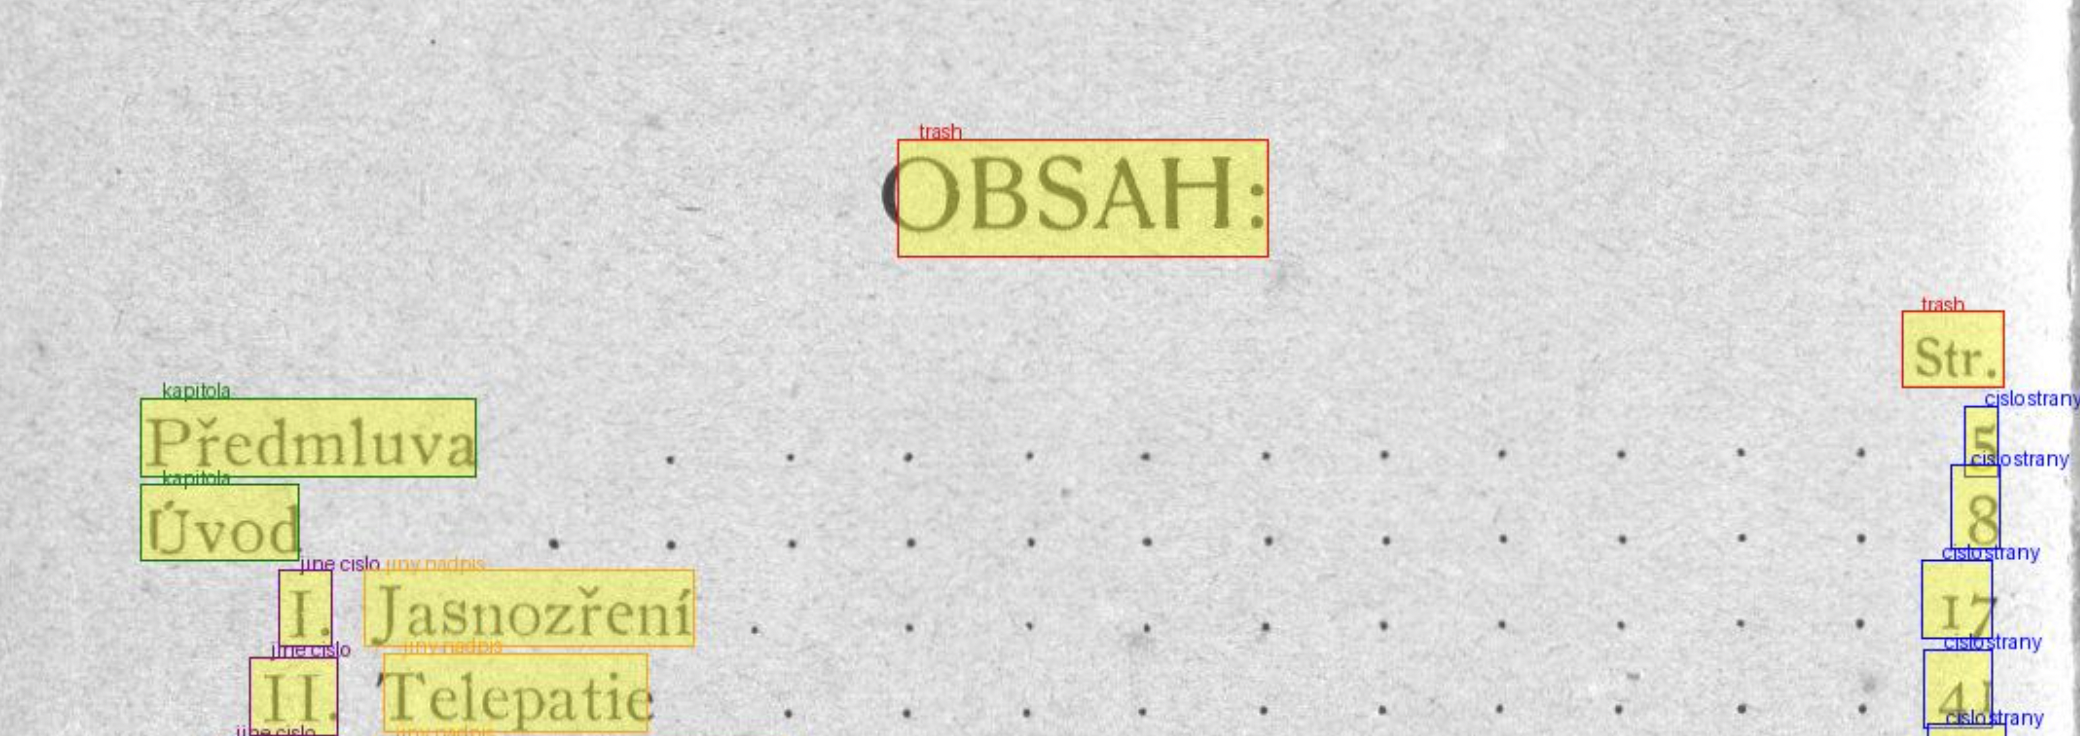
\includegraphics[width=1\linewidth]{img/layout-input-inlustration.png}
    \caption{Vizualizace výřezu výstupu z LayoutLMv3 včetně vyznačených klasifikací. Tento bod slouží k ověření, že práce se souřadnicemi pomocí normalizace/denormalizace probíhala korektně a že jednotlivá slova jsou klasifikována správně.}
    \label{fig:layout-output}
\end{figure}

V tomto kroku se ale také projevuje hlavní nevýhoda LayoutLMv3, a to ta, že vstup je omezen na pouhých 512 tokenů. Tento problém byl částečně vyřešen tak, že v případě delšího vstupu je vstup rozdělen na několik částí a jednotlivé části prochází modelem sekvenčně. Tento přístup funguje v pořádku s většinou vstupů, ovšem jsou zde i případy, kdy nepřítomnost celého kontextu strany vede ke špatné klasifikaci. Příklady takového zpracování lze vidět na obrázcích \ref{fig:layout_good} a \ref{fig:layout_bad}.

\begin{figure}[h!]
    \centering
    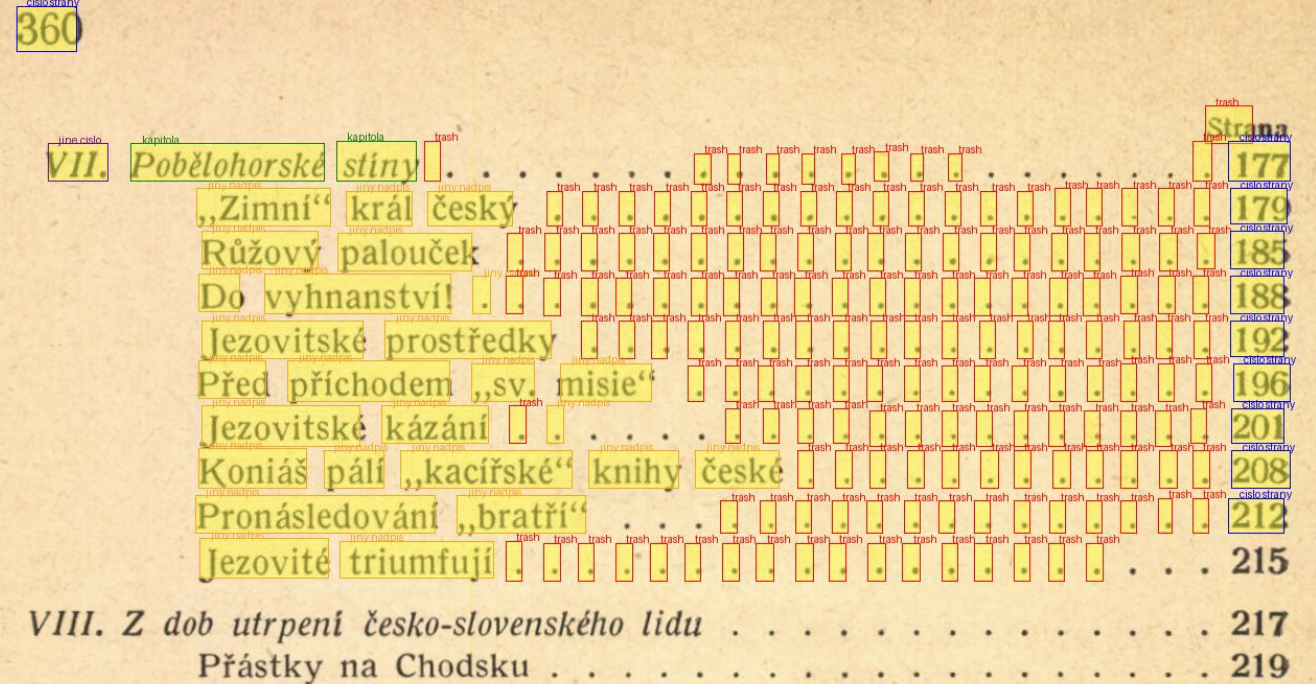
\includegraphics[width=\textwidth]{img/layout_good.png}
    \caption{První zpracovaná dávka strany. Všechna slova (kromě některých teček) jsou zde označena korektně, správně jsou rozlišeny kapitoly od podkapitol.}
    \label{fig:layout_good}
\end{figure}

\begin{figure}[h!]
    \centering
    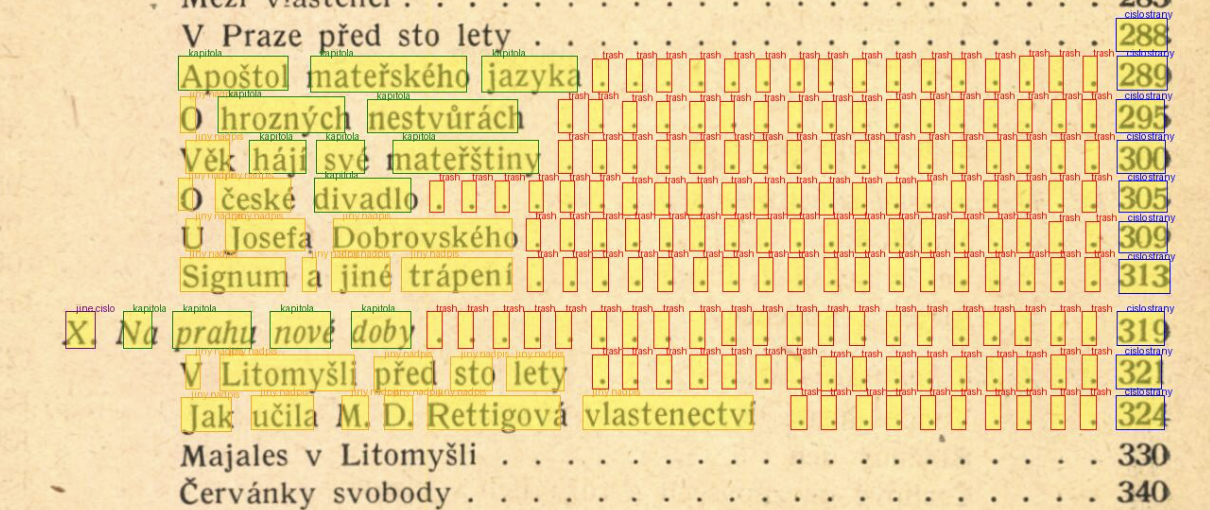
\includegraphics[width=\textwidth]{img/layout_bad.png}
    \caption{Čtvrtá zpracovaná dávka strany. U této dávky model již ztratil kontext o předcházejících kapitolách, proto nesprávně klasifikuje podkapitoly jako kapitoly a zkalibruje se až po další opravdové kapitole.}
    \label{fig:layout_bad}
\end{figure}

\newpage


\subsubsection{Převod výstupů do formátu JSON}

Pro potřeby inference máme k dispozici data z OCR: slova, jejich bounding boxy a klasifikace jednotlivých slov. Následující pipeline představuje výsledek řady experimentů a kompromisů s cílem zpracovat tato data co nejkorektněji pro širokou škálu vstupů/dokumentů.

Během implementace jsme zvažovali různé přístupy, například průchod po řádcích podle formátu ALTO (výstup PERO-OCR). Tímto postupem lze v ideálním případě získat slova uspořádaná podle logických řádků, což je zpravidla požadovaný výstup. Ukázku ideálního vstupu pro tento přístup ilustruje obrázek \ref{fig:img_textblock_adv}. Tento přístup však nelze spolehlivě použít u různorodých dokumentů, protože výstup OCR (ve formátu ALTO) text často dělí na tzv. \texttt{TextBlocks}, které v mnoha případech odpovídají spíše sloupovému rozvržení (např. nadpis, číslo strany a kapitoly umístěné vedle sebe), nikoli logickým řádkům, jak ukazuje obrázek \ref{fig:img_textblocks_dis}. Jednoduchý průchod po "řádcích" definovaných těmito bloky je pak problematický.

\begin{figure}
    \centering
    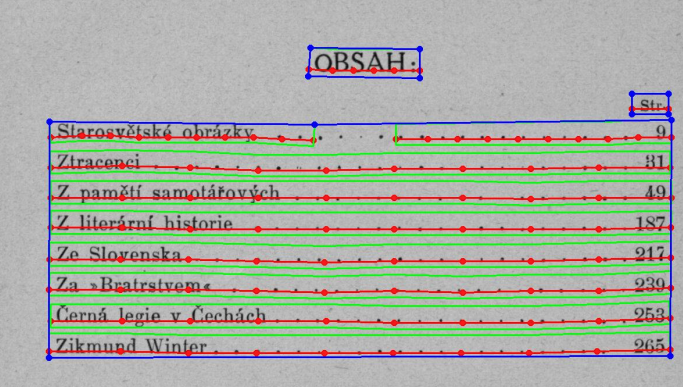
\includegraphics[width=1\linewidth]{img/textblock_adv.png}
    \caption{Ukázka vstupu vhodného pro zpracování po řádcích podle výstupu OCR.}
    \label{fig:img_textblock_adv}
\end{figure}

\begin{figure}
    \centering
    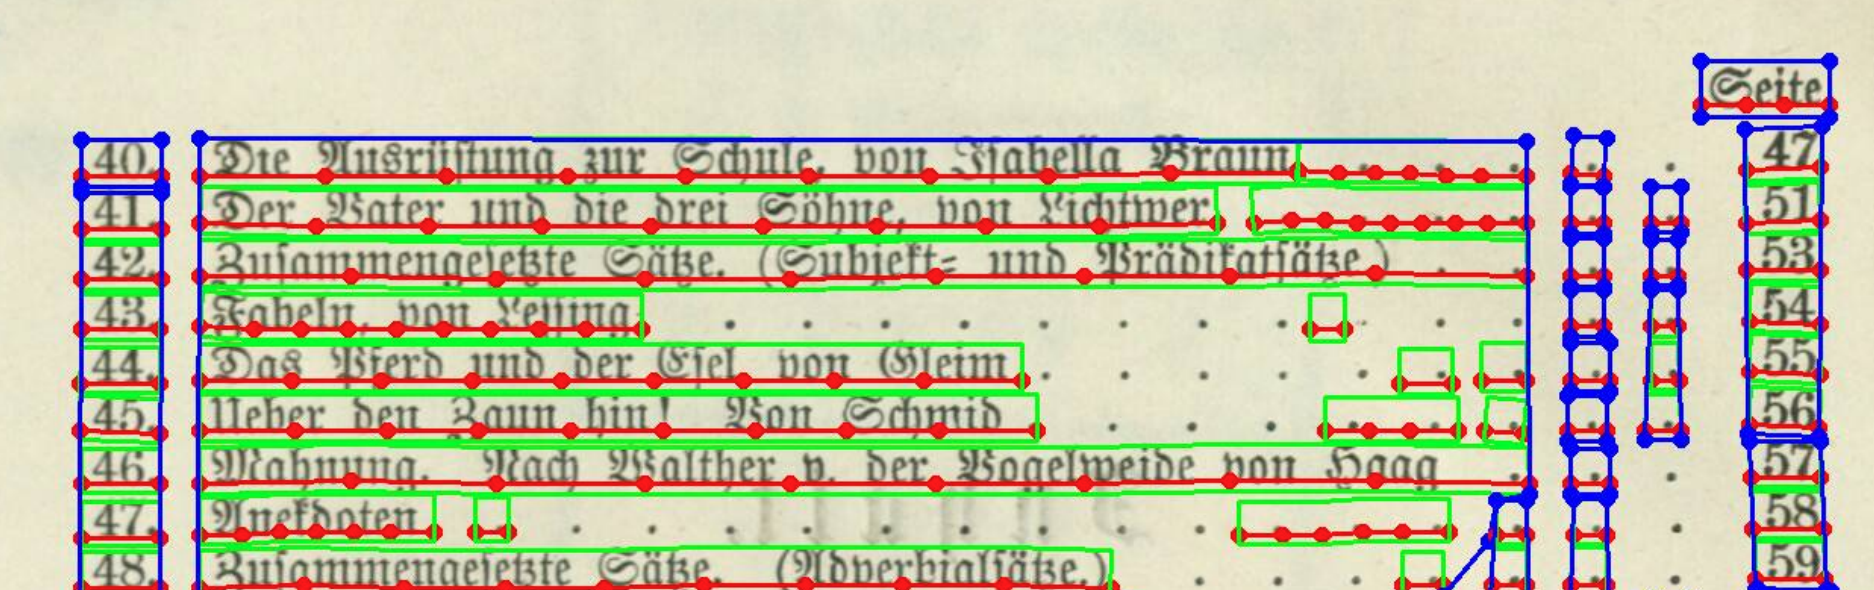
\includegraphics[width=1\linewidth]{img/textblocks_dis.png}
    \caption{Ukázka nevhodně rozdělených \texttt{TextBlock} bloků (znázorněno modře) znemožňující průchod po logických řádcích podle výstupu OCR.}
    \label{fig:img_textblocks_dis}
\end{figure}

Dalším problémem byla spolehlivá detekce jedno- či víceřádkových nadpisů a tomu odpovídající parsování. Zkoušeli jsme různé přístupy, například zjišťování, zda další řádek začíná odsazeně vzhledem k předchozímu, ale to nefungovalo příliš dobře. Nespolehlivým se ukázalo i získávání této informace podle toho, zda daný řetězec má v blízkosti číslo kapitoly, především proto, že ne všechny nadpisy mají v těsné blízkosti čísla kapitol.

Značné potíže působilo také určení, zda k danému nadpisu náleží číslo stránky a kapitoly, a pokud ano, ke kterému konkrétnímu nadpisu. Pokusy přiřadit čísla k nejbližšímu nadpisu selhaly. To se ukázalo jako nespolehlivé především kvůli proměnlivé délce nadpisů (jednorádkové vs. víceřádkové), sloupovému rozvržení a dalším faktorům, které ovlivňovaly výpočet "nejbližšího".

Po důkladné analýze výstupů a řadě experimentů se zpracováním jsme dospěli k závěru, že pro široce různorodé dokumenty není možné v rámci tohoto projektu navrhnout čistě pravidlový systém, který by fungoval spolehlivě bez významných kompromisů. Řešením by bylo buď jasné vymezení vstupní domény (např. co do počtu sloupců, struktury nadpisů atd.), nebo využití technik strojového učení pro extrakci dat do JSONu. To by mohla být klasifikace typů obsahu (nadpis, odstavec, číslo) nebo kompletní end-to-end model. Tyto přístupy však nebyly předmětem/cílem tohoto projektu, a proto nebyly implementovány.

Výsledný (implementovaný) přístup se proto snaží minimalizovat kompromisy a dosáhnout rozumné funkčnosti pro co nejširší spektrum vstupů. Skládá se z následujících kroků:
\begin{enumerate}
    \item Filtrace relevantních slov (např. nadpisů, čísel stran, čísel kapitol) na základě jejich klasifikace.
    \item Spojování jednotlivých slov do vět (víceslovné nadpisy, víceciferná čísla atd.).
    % mám nachystane to dělat přes ty alto ale zatím jsem to nedodělal
        \begin{enumerate}
            \item Vybraná slova se zpracovávají podle jejich klasifikace.
            \item Pro slova v rámci stejné třídy se provede pokus o spojení. Slova se spojí, pokud leží na přibližně stejné horizontální úrovni a jejich horizontální vzdálenost (včetně mezery) nepřesahuje určitou mez. Tato mez je relativní vzhledem k výšce bounding boxu slova (de facto výška řádku).
            \item Postup se opakuje, dokud nejsou zpracována všechna slova dané třídy/všechen relevantní text.
        \end{enumerate}
    \item Vytvoření relací mezi nadpisy a příslušnými čísly stran či kapitol (pokud existují).
        \begin{enumerate}
                \item Pro každý nadpis se určí jeho horizontální středová linie.
                \item Pro každé slovo klasifikované jako číslo strany nebo číslo kapitoly se zjistí, zda jeho vertikální rozsah (bounding box) protíná horizontální středovou linii některého nadpisu.
                \item Mezi protínajícími se kandidáty (čísly) a daným nadpisem se spočítá euklidovská vzdálenost jejich středů (zvlášť pro čísla stran a zvlášť pro čísla kapitol).
                \item Jako příslušné číslo (strany/kapitoly) je vybrán ten kandidát s nejmenší euklidovskou vzdáleností od nadpisu.
        \end{enumerate}
    \item Určení nadřazeného (hlavního) nadpisu pro dané (pod)nadpisy na základě horizontální blízkosti či odsazení.
    \item Sestavení výsledného JSON objektu z extrahovaných a propojených informací.
\end{enumerate}

\section{Vyhodnocení přístupu s LayoutLMv3 }
Pro vyhodnocení jsme si napsali script dostupný v odevzdaném repozitáři. Tento script porovnal GT JSON souborů\footnote{Získané LLM a validované ručně} s hodnotami predikovanými pipline modelu LayoutLMv3. Pro porovnání s DONUT modelem jsme použili stejný dataset jako pro validaci DONUTu a taktéž nás zajímalo průměrné TED skoré a F1 skoré. Obě tyto hodnoty jsou počítany maximálně podobným způsob jak v modelu donut. Bohužel uplně přesně stejného výpočtu nejde dosáhnout, protože v DONUT modelu jsou hodnoty metrik počítané před konverzí strukturovaného výstupu na JSON. 

\begin{table}[htp]
\centering
\begin{tabular}{c||cc}
\hline
\textbf{Počet epoch LayoutLMv3} & \textbf{Norm. tree edit distance přesnost} & \textbf{F1 skóre} \\
\hline
10 & 0.73 & 0.19 \\
\hline
\end{tabular}

\caption{Tabulka s výsledky inference pipline založené na LayoutLMv3.}
\label{tab:layout_rez}
\end{table}

Pro lepší pochopení dat jsme si vykreslili histogram rozložení na obrázku \ref{fig:layout_histogram}. Z rozložení dat je zjevné, že navržený systém funguje relativně dobře. Vysoká přesnost TED indikuje, že se systému relativně dobře daří 
předpovídat strukturu, což ale není příliš překvapivé, protože dataset 
obsahuje relativně jednoduché obsahy. Dále pak proto, že jsou málo časté
 kombinace vícesloupcových či víceřádkových nadpisů, u kterých víme, že 
je systém náchylný k chybám, které v datasetu téměř nejsou. Mimo to má 
systém předpovídání struktury značně jednodušší, protože struktura se 
nemusí hádat, ale pouze "nasazuje" na získané informace.


Nízká přesnost F1 naproti tomu jasně 
ukazuje na nedokonalý postprocessing, který, jak jsme nastínili dříve, 
by šlo vylepšit pouze za cenu obrovské komplexity nebo použitím 
principiálně jiného modelu.
\begin{figure}[h!]
    \centering
    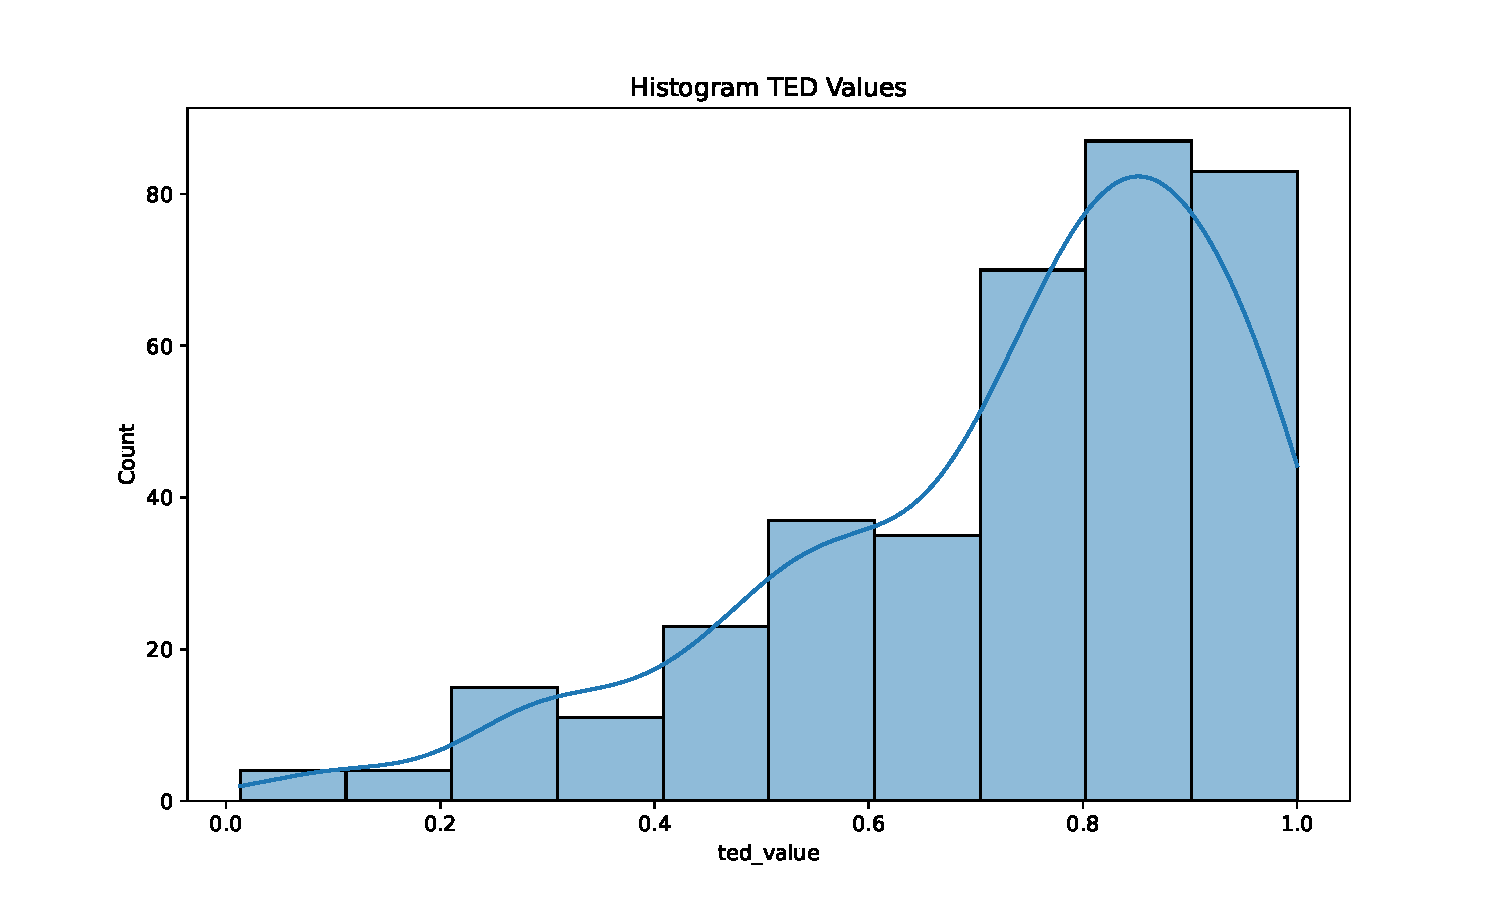
\includegraphics[width=1\linewidth]{img/ted_histogram.pdf}
    \caption{Histogram rozložení TED hodnot v datasetu. }
    \label{fig:layout_histogram}
\end{figure}

\newpage
\section{Závěr}
% TOHLE JE NAVRH 
Cílem tohoto projektu bylo prozkoumat a implementovat systémy pro automatické zpracování skenovaných stránek s obsahem knih a dokumentů a extrakci strukturovaných informací o kapitolách, jejich číslech, číslech stránek a hierarchickém vztahu. Pro dosažení tohoto cíle jsme se zaměřili na dva hlavní přístupy: end-to-end model založený na architektuře Transformer (DONUT) a sekvenční řešení kombinující optické rozpoznávání znaků (PERO OCR) s modelem pro porozumění dokumentům založeným na rozložení naskenované strany (LayoutLMv3).

Pro model DONUT jsme se rozhodli pro přístup k tvorbě anotací pomocí velkého jazykového modelu (LLM). V druhé části semestru jsme zvalidovali přesnost dat pro validaci přesnosti. Data pro PERO OCR + LayoutLMv3 přístup vyžadovala jiný typ anotací, zaměřený na klasifikaci slovních tokenů na základě jejich pozice a bounding boxů, což představovalo odlišné výzvy.


Oba přístupy jsme vyhodnotili pomocí standardních metrik -- normalizované Tree Edit Distance a F1 skóre. I přes počáteční potíže s adaptací modelu DONUT, který nebyl trénován na českém jazyce, a nutnost úprav jeho kódu pro dosažení stabilních výsledků trénování, model DONUT v našem testování dosáhl pro danou úlohu lepších výsledků ve srovnání s řešením PERO OCR + LayoutLMv3.

Závěrem lze říci, že ačkoliv přístup založený na PERO OCR a LayoutLMv3 poskytuje detailní klasifikaci na úrovni slov a mohl by být užitečný pro jiné úlohy zpracování dokumentů, pro extrakci strukturovaného obsahu z obrazových dat se v rámci tohoto projektu ukázal jako efektivnější model DONUT. Primární problém PERO + LayoutLMv3 řešení totiž leží v posledním kroku zpracování, kdy je výstup modelu přetvářen na výstupní JSON, který nelze s dostatečnou přesností rozumně realizovat pomocí standardního programování. Proto pro další možné směry, kterými by se toho řešení mohlo ubírat, by mohlo být např. vyzkoušení natrénování neuronové sítě pro sestavení výstupů. 

End-to-end povaha našeho baseline modelu DONUT a možnost rychlé tvorby dat s asistencí LLM, byť s nutností ruční kontroly, představovala jednodušší cestu pro řešení úloh porozumění dokumentům přímo z jejich obrazové reprezentace. Navíc, DONUT bylo možné trénovat na větším datasetu z důvodu nepotřeby anotací, a díky tomu jsme jej také mohli trénovat na stránkách s více než dvojúrovňovým zanořením obsahů.


\newpage
\bibliographystyle{alpha}
\bibliography{sample}

\end{document}